In this appendix we will illustrate basic mathematical tools used all through the thesis.
They are shown here because without been figures of merit of the conceptual parts involving this thesis, they are nowadays sufficiently important for any whose intention is t expertise on this field of Quantum Metrology and Quantum Information.

\subsection{Husimi Q-representation and the Bloch sphere}

To represent states of total angular momentum bigger than $\frac{1}{2}$ we use the Husimi quasi-probability on the $\bs{n}$ unitary vector space defined as $2+2$
\be
  Q(\alpha) = \braopket{}{\varrho}{\alpha}
\ee
where ...

It is very common to express the particle density.

\subsection{Discussion on angular momentum subspaces for different spins}
\label{app:angular-subspaces}

Here we want to show how the whole Hilbert space of the spin angular-momentum of a multi-particle system is structured.
When same kind of spin-$j$ particles, i.e., qubits or qudits on the Quantum Information framework, are the constituents of the system, several important properties and structures arise.
We will explain how these Hilbert spaces are added to form a larger Hilbert space while we describe the notation used in this thesis.

First of all, we have the basic single particle $d$-level system or qudit.
When $d$ equals two we have the well known 2-level system or qubit.
The basis of such systems have $d$ eigenstates of the spin operator $j_z^{(n)}$, where $n$ stands for the particle label and the spin number $j$ is in each case $(d-1)/2$.
Just to remind that $j$ integer stand for bosonic systems whereas $j$ half integers for fermionic systems.
So to say the eigenstates are characterized by
\be
  j_z^{(n)}\ket{m} = m \ket{m}
\ee
for $m = -j,-j+1,\dots,+j-1,+j$.
It is clear that in Quantum Information the two eigenstates $\ket{-1/2}$ and $\ket{+1/2}$ of 2-level systems, or qubits, are identified with $\ket{0}$ and $\ket{1}$ respectively, since the qubit case is the most studied case on which the dichotomized representation of classic \emph{bit}s, ones and zeros, is directly related with.

When adding particles into a bigger system convenient representation is key to compute efficiently.
A first approach is to add all eigenstates one after the other and permute the states from right to left,
\be
  \begin{split}
    & \ket{-j,-j,\dots,-j,-j},\\
    & \ket{-j,-j,\dots,-j,-j+1},\\
    & \vdots \\
    & \ket{-j,-j,\dots,-j+1,-j},\\
    & \ket{-j,-j,\dots,-j+1,-j+1},\\
    & \vdots \\
    & \ket{+j,+j,\dots,+j,+j},
  \end{split}
\ee
where we have used the notation $\ket{m_1,m_2,\dots,m_{N-1},m_N}\equiv \ket{m_1}\otimes\ket{m_2}\dots\otimes\ket{m_N}$.
This basis is still an eigenbasis of $J_z = \sum_{n} j_z^{(n)}$, the total angular momentum $z$ component.
On the other hand, it is not a eigenbasis of the total angular momentum $\bs{J}^2 = J_x^2+J_y^2+J_z^2$ neither they are permutationally invariant, i.e., (anti)symmetric, states.
So a more convenient representation is explained here.

We will explain shortly how to construct a basis on which all states from the basis are eigenstates of the total angular momentum $\bs{J}^2$, see Ref.~\citep{}.
For that, we have the $J_{\pm} := J_x \pm i J_y$ operators which increase or decrease eigenvalue of $J_z$ without changing the eigenvalue of $\bs{J}^2$.
Therefore, if we start from $\ket{-j,-j,\dots,-j}$, which is an eigenstate of $\bs{j}^2$ with the maximal eigenvalue $Nj(Nj+1)$, and we apply $J_+$ subsequently we obtain all the states belonging to this subspace on which $\bs{J}^2$ is maximal \citep{}.
We keep doing this until we have all the subspaces characterized.
The eigenbasis can be characterized with three simple numbers $\ket{J,M,D}$, the total angular momentum number, the angular momentum projection quantum number into the $z$-direction, $M=-J,-J+1,\dots,+J-1,+J$, and the degeneracy number of the $J$ subspaces, $D=1,2,dots,D_J$.

We now show the definition of some of the most used states throughout this thesis.
For the spin-$\frac{1}{2}$ particles, i.e., qubits, several states arose.
We have all the symmetric states where $m$ particles are in the $\ket{1}$ state and the rest $N-m$ are in $\ket{0}$.
Since the symmetric subspace is not degenerated in this case we omit the degeneracy number
\be
  \begin{split}
    \ket{J=N/2,M=N/2} & \equiv \ket{1,1,1,\dots,1,1}, \\
    \ket{N/2,N/2-1} & \equiv N^{-1/2}\sum_k \mathcal{P}_k(\ket{1}\otimes \ket{0}^{\otimes{N-1}}), \\
    \vdots &\\
    \ket{N/2, M} & \equiv \binom{N}{N/2-M}^{-1/2}\sum_k \mathcal{P}_k(\ket{1}^{\otimes{N/2-M}}\otimes\ket{0}^{\otimes N+M-N/2}), \\
    \vdots&\\
    \ket{N/2,-N/2} & \equiv \ket{0,0,0,\dots,0,0},
  \end{split}
\ee
where the sums appearing are over all possible different permutations of the state $\mathcal{P}_k$.
Notice the similarity with respect to the Dicke states Eq.~\eqref{}.
Later on we will show the connection with the Dicke states.

For now, we present another well known state, the permutationally invariant singlet for spin-$\frac{1}{2}$ qubits.
This state has been recently found to be unique and therefore it has been able to rewrite it in several ways \citep{}.
The first most trivial definition is that it is permutational invariant ground state of $H=\bs{J}^2$, from which it can be written as the thermal state at zero temperature for such a Hamiltonian. The second definition is that the PI singlet can be written also as the equally weighted mixture of all the degenerated singlets, i.e., $\ket{J=0,M=0,D}$ for $D=1,2,\dots,D_0$.
An the last definition comes from mixing all the possible permutations of the product of pairwise singlets, $\ket{\Psi^-}:=\frac{1}{\sqrt{2}}(\ket{1}\otimes\ket{0}-\ket{0}\otimes\ket{1})$.
Finally, we write those equivalences
\be
  \lim_{\beta\rightarrow\infty}\frac{\exp(-\bs{J}^2\beta)}{\tr(\exp(-\bs{J}^2\beta))}\equiv \frac{1}{D_0}\sum_{D=1}^{D_0}\ketbra{0,0,D}{0,0,D} \equiv \sum_{k}\mathcal{P}_k(\ketbra{\Psi^-}{\Psi^-}^{\otimes{N/2}})
\ee

\subsection{Legendre transform}
\label{app:legendre-transform}

The Legendre transform of a convex function, say $f:x \rightarrow f(x)$, is defined as the maximum distance between the function the line $rx$ and $f(x)$ at same $x$.
In can be written as follows,
\be
  \hat{f}(r):=\max_{x}\{rx-f(x)\},
\ee
where $\hat{f}(r)$ represents the transformed function~\citep{Rockafellar1996}.
A geometric representation of the transform is given on the Figure~\ref{fig:lt-geometric-legendre}.

\begin{figure}
  \centering
  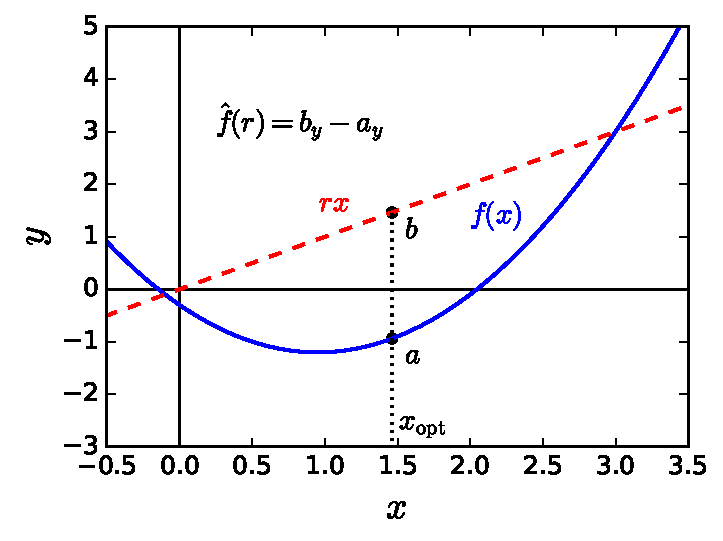
\includegraphics[scale=.65]{img/plots/LT_legendre.pdf}
  \caption[Graphical representation of the Legendre trasnform.]{Graphical representation of the Legendre transform. (blue-line) Convex function, $f(x)=x^2-1.9x-0.3$, to be transformed. (red-dashed) Constant slope line passing by the coordinate system origin, $rx$. The Legendre transform is the maximal difference between $rx$ and $f(x)$ at the same $x$. In this case, the vertical distance between $a$ and $b$.}
  \label{fig:lt-geometric-legendre}
\end{figure}

The inverse transformation is simply obtained by applying again the same technique.
One fully recovers the
\be
  f(x) = \max_{r}\{rx-\hat{f}(r)\}.
\ee

Let us develop the example shown in the Figure~\ref{fig:lt-geometric-legendre}, where the function is $f(x)=x^2-1.9x-0.3$.
In this case the problem is well defined on the complete real axis.
Now, one has to find the maximum of $g(r,x)=rx-f(x)$ for all $\forall r$.
This maximum is easily obtained in this particular case with usual techniques.
On has to solve for x the following equation $\partial_x g(r,x) = 0$. Thus, the maximum is at $x_{\text{opt}} = \frac{r+1.9}{2}$ and hence, the Legendre transform is the following,
\be
  \hat{f}(r) = \frac{r^2}{4}+0.95r+1.2025.
\ee
If one applies again the transformation the resulting function is again the original one.

\subsubsection{Binomial identities}
